\documentclass[11pt,letterpaper]{article}
\usepackage{pslatex}
\usepackage[english]{babel}
\usepackage[utf8]{inputenc}
\usepackage{latexsym}
\usepackage{amssymb} 
\usepackage{amsmath}
\usepackage{epsfig}
\usepackage{hyperref}

\usepackage{url}
\graphicspath{ {../planning/} }
\begin{document}

\pagestyle{empty}

\title{
    Hardware-accelerated similarity search indices on the Adapteva Parallella-16 reconfigurable computing machine
}
\author{
Erik Regla (Student)\\
Rodrigo Paredes (Advisor)\\
Civil Computer Engineering\\ 
University of Talca}
\date{\today}
\maketitle

\section{Proposal description}

\subsection{Project's context} 

    With the current advances in transistor technology, the design of 3D layered silicon chips and 5nm 
    lithography, Moore's Law is now a problem as now is harder to push the hardware limits -for single chips-
    at the same rate as ten years ago\cite{7478302,EETIMES1}. As stated in an 2007 technical report made by Altera
    Corporation: \emph{``For most of the microprocessor's history, application demands have risen in response to 
    processor improvements, allowing processors to stay ahead of demand. In the last few years, however, the 
    situation has changed. High-performance computing (HPC) applications are now demanding more than processors 
    alone can deliver, creating a technology gap between demand and performance.''}\cite{ALTERA_Accel_fpga}


    This \emph{Technology gap} is nowadays tackled by the using of heterogeneous computer architectures, being
    General Purpose GPU Computing (GPGPU) one of the most recurrent solutions due to the ease of programming
    and solution design provided by hardware-specific programming languages like Nvidia CUDA
    \cite{NVIDIA_volta}. But even promising solutions like GPGPU have their shortcomings, as energy consumption
     and branch divergence heavily degrades performance on control-flow intensive algorithms
    -which are the most common- \cite{6376229}.


    There is a growing interest on \emph{high-performance and low-power custom computing machines} which 
    aim to design \emph{Application-specific integrated circuits} (ASICs) in order to solve certain 
    computational problems. But as ASIC design, prototyping, and implementation is very costly,
    \emph{Field Programable Gate Arrays} (FPGAs) has been proven as a cost-effective solution to implement those 
    designs and interconnect them with our current platforms to form reconfigurable computing architectures
    \cite{ReconfigurableComputing, 6589302,Compton00anintroduction} being only limited by their power-budget while offering 
    a scalable compute model for certain problems even after Moore's law end.

\subsection{Problem definition} 
    One of the many approaches to perform similarity searches is to perform k-nn or range queries on permutant-based 
    indices, which abstract the dataset dimensionality and the cost of the object-object distance calculation. To 
    perform a search on this index, a permutation is generated for the query object and then compared to the whole 
    dataset under the premise that computing distance between two permutations is faster than computing the full 
    distance between the two elements. After their distances are computed, a subset is selected under a certain 
    criteria given by the query nature and the results are filtered later in order to answer the query.
    \cite{5271946,5271944}


    As permutations are abstractions of the intrinsic dataset dimension, as we reduce the permutation/dimensionality 
    ratio, the results become inaccurate, on the other hand, if we raise the ratio to increase accuracy we end 
    processing the whole dataset rendering the approach useless as it's more time consuming than the original 
    problem.

    This behaviour makes similarity search indices a perfect test bench for its implementation on a reconfigurable
    computing device\cite{5999889} such as the Adapteva Parallella-16, a \emph{System on chip} (SoC) based on the 
    Xilinx All Programmable Zynq7000 Series SoC which packs a Dual-core 32-bit ARM Cortex-A9 host controller and a 
    Artix-7 FPGA \cite{DBLP:journals/corr/OlofssonNZ14,LINLEY_1}.
    The board also has an Epiphany III multicore accelerator coprocessor, interconnected with the host-controller
    though an FPGA designed ASIC in order to be used as a low-power high-performance heterogeneous computing 
    platform.

    The main problem with reconfigurable computing is the complexity of circuit design \cite{SPA_thesis}. 
    Independently of the algorithm being ported to an FPGA implementation, there is not automated way to use
    the same source code used on the Processing System (PS) version of the problem in the Programmable Logic (PL). 
    As there are some tools developed for both FPGA manufacturers and 3rd parties to design circuits using the C 
    language, they lack of precision and many considerations and ``compile'' optimizations must be performed 
    in order to successfully port certain algorithms\cite{SPA_thesis}, such as instruction pipelines, read/write 
    syncronization, clock gating\cite{XILINX_clockgating}, etc \cite{XILINX_axi,XILINX_clockgating,
    XILINX_ddr_rate,XILINX_mem_interface}.
\subsection{Current works} 
    Alvarez \cite{SPA_thesis} implemented a positioning system based on video streams using a Dilligent Zedboard 
    \cite{DILLIGENT_zedboard_reference}. In this implementation, an FPGA accelerator were used to increase the 
    image processing throughput by interfacing the camera input to a series of filters by using an AXI4 interface.
    The FPGA implementation increased eight times the original processing rate for 1080p video streams despite not 
    being performed any code optimizations, correct pragmas, or hardware replication.\cite{XILINX_hls_ultrafast}.

    Rodriges \cite{BR_thesis} developed an operating infrastructure on a Parallella-16 board, but in this work
    the FPGA is used in the same way as the original developers intended, to interconnect the components of the
    board in a custom way \cite{DBLP:journals/corr/OlofssonNZ14}, but no acceleration hardware were designed at this
    point.

    Olofsson \cite{PARALLELLA_accelerator} explained how to create FPGA accelerators but the examples provided
    in their repository are not functional. Olofsson also states that building accelerators on FPGAs is a
    time-consuming work with a high \emph{mistake cost} \cite{PARALLELLA_accelerator}. 
    
\subsection{Proposed solution}
    In order to accelerate a similarity search engine, we will develop a naive implementation of a 
    permutant-based metric space index without any major optimizations to study the feasibility of porting
    each subroutines involved based on their potential parallelism.

    Some of the target routines to evaluate include incremental sorting routines\cite{7416566}, permutant generation 
    and comparison\cite{5271946} and massive distance calculations \cite{5271944,5271946}, as those operations
    are expected to be executed in a pipelined fashion.

    After the study, we will port such algorithms as Intellectual Properties (IPs) though the use of Xilinx Vivado 
    HLS to be validated and then implemented on the FGPA as accelerators for further interconnect with the 
    host-controller \cite{SPA_thesis, XILINX_hls_design_guide, XILINX_hls_reference, XILINX_software_guide, 
    XILINX_hls_design_tuto, XILINX_hls_ultrafast}. Then a performance comparison will be executed in order to 
    determine the success of the solution and to prove if Olofsson statements regarding FPGA computing
    \cite{PARALLELLA_accelerator} on the Adapteva Parallella platform were correct or not.


\section{Objectives}
\paragraph{Main objective}
\begin{itemize}
\item Study the feasibility of implementing hardware-based accelerators for the Adapteva Parallella SoC.
\end{itemize}

\paragraph{Specific objectives}
% \emph{(Una lista de puntos que detallan el objetivo general.)}
\begin{itemize}
    \item Specify requirements and considerations to be accounted when porting general purpose algorithms to FPGAs.
    \item Study and implement a PL-PS data sharing sharing solution.
    \item Develop a functional FPGA-based hardware-accelerator prototype for a subset of routines involved 
    on approximate similarity search.
    \item Deliver a solid guide to serve as a starting point to future computer scientists with little or no 
    knowledge about hardware design. 
\end{itemize}



\section{Scope}
\begin{itemize}
    \item During this work we will not create a framework to develop new algorithms on FPGAs. 
    \item Also, we will not work on optimizations for the original versions of the tested routines.
    \footnote{This is because we expect to obtain a performance boost by implementing the same algorithms as ASICs.}
    \item This work is limited only to research about FPGA hardware design, and to compare and contrast both 
        software and hardware implementations on a Adapteva Parallella-16 SoC.
\end{itemize}



\section{Methodology}

\paragraph{Milestone 1:} ``Approximate search algorithms and indices"
\begin{itemize}
    \item Analyse previously developed hardware-accelerators.
    \item Research about resource sharing methods and techniques for the proposed architecture.
    \item Implement a simple hardware-accelerator IP Core on the FPGA.
    \item Study possible problems which could arise when porting common algorithms on custom hardware.
    \item Research about approximate search indices for metric spaces.
    \item Research about workarounds for high-dimensionality metric space datasets.
    \item Implement a permutant-based index and query algorithm.
    \item Analyse the behaviour of the implemented solution and identify potential targets for hardware-acceleration
\end{itemize}

\paragraph{Milestone 2:} ``Hardware-accelerated index implementation"
\begin{itemize}
    \item Research about hardware prototyping.
    \item Research about hardware-software interconnection techniques and technologies applicable to the
    target platform. 
    \item Implement as IP Cores the selected code fragments.
    \item Implement an interconnection protocol for resource sharing between the two platforms.
    \item Detect possible bottlenecks or other problems derived from the interconnection between the Atrix-7 
    FPGA and the ARMv7 A9 processor.
    \item Implement a loadable bitstream for the Parallella board and design according kernel modules.
    \item Replace software solution with custom hardware solution.
    \item Benchmark hardware implemented solution and contrast it with software implementation.
\end{itemize}

\section{Work plan}
\begin{figure}[!ht]
    \centering
  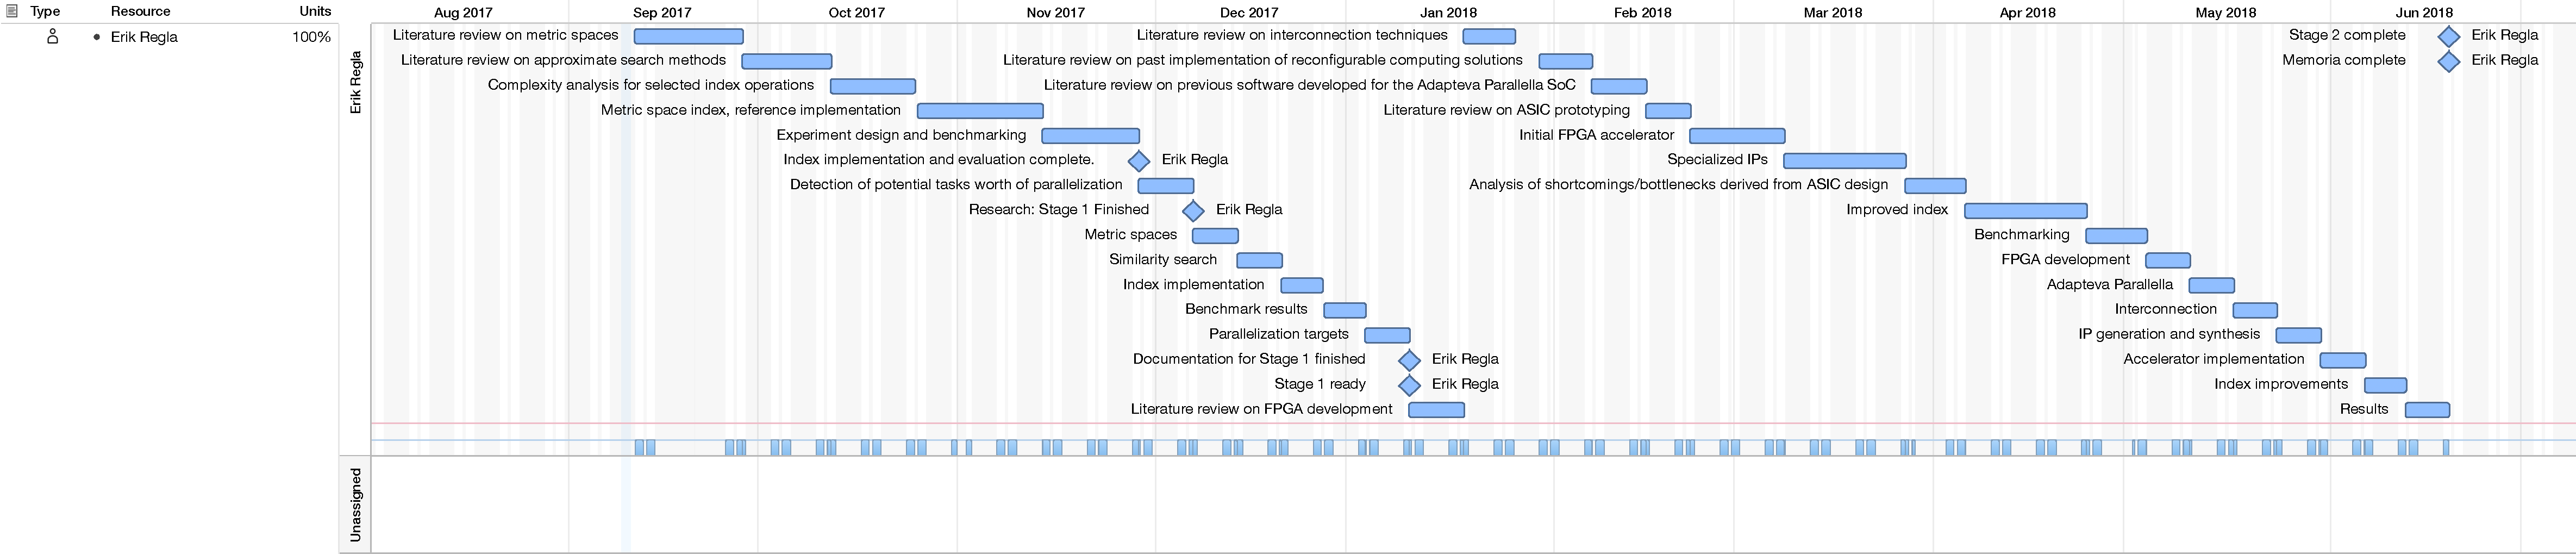
\includegraphics[scale=.15]{initial_planning_time_outline} 
    \caption{Work plan schedule}
    \label{FIGURE:WORKPLAN}
  \end{figure}

\bibliographystyle{plain}
\bibliography{referencias}


\end{document}